\begin{frame}{PageRank e Centralidades}
    \framesubtitle{Identificação de Atletas Estruturalmente Importantes}
    \begin{block}{Objetivo}
        Identificar atletas de maior importância estrutural nas redes competitivas através de métricas de centralidade.
    \end{block}

    \begin{columns}[T]
        \begin{column}{0.48\textwidth}
            \textbf{Métricas Calculadas:}
            \begin{itemize}
                \item \textbf{PageRank}: Importância global
                \item \textbf{Betweenness}: Atletas-ponte
                \item \textbf{Closeness}: Proximidade
                \item \textbf{Degree}: Conexões diretas
            \end{itemize}
        \end{column}
        \begin{column}{0.48\textwidth}
            \textbf{Achados Principais:}
            \begin{itemize}
                \item Michael Phelps: PageRank 0.027
                \item 14/20 top atletas são mulheres
                \item Atletas-ponte: 10.2\% (natação)
                \item Métricas revelam padrões ocultos
            \end{itemize}
        \end{column}
    \end{columns}
\end{frame}

\begin{frame}{Top 10 Atletas por PageRank - Swimming}
    \framesubtitle{Ranking Estrutural vs. Contagem de Medalhas}
    \begin{table}[h]
        \centering
        \footnotesize
        \begin{tabular}{clccc}
            \toprule
            \textbf{Rank} & \textbf{Atleta} & \textbf{País} & \textbf{PageRank} & \textbf{Medalhas} \\
            \midrule
            1 & Michael Phelps & USA & 0.0270 & 28 \\
            2 & Natalie Coughlin & USA & 0.0189 & 12 \\
            3 & Dara Torres & USA & 0.0177 & 12 \\
            4 & Jenny Thompson & USA & 0.0171 & 12 \\
            5 & Ryan Lochte & USA & 0.0149 & 12 \\
            6 & Matt Biondi & USA & 0.0138 & 11 \\
            7 & Allison Schmitt & USA & 0.0131 & 10 \\
            8 & Missy Franklin & USA & 0.0125 & 7 \\
            9 & Ian Thorpe & AUS & 0.0115 & 9 \\
            10 & Dawn Fraser & AUS & 0.0110 & 8 \\
            \bottomrule
        \end{tabular}
    \end{table}
    \vspace{-0.3cm}
    \begin{block}{}
        \footnotesize
        PageRank captura não apenas número de medalhas, mas \textbf{qualidade dos competidores} enfrentados.
    \end{block}
\end{frame}

\begin{frame}{Diferenças por Gênero}
    \framesubtitle{Estrutura das Redes Masculinas vs. Femininas}
    \begin{block}{Observação Principal}
        Predominância feminina no top 20 global (14/20) reflete \textbf{estrutura diferenciada} das redes, não superioridade absoluta.
    \end{block}

    \begin{columns}[T]
        \begin{column}{0.48\textwidth}
            \textbf{Redes Femininas:}
            \begin{itemize}
                \item Menor número de competidoras
                \item Maior concentração de PageRank
                \item Valores individuais mais altos
                \item Estrutura mais centralizada
            \end{itemize}
        \end{column}
        \begin{column}{0.48\textwidth}
            \textbf{Redes Masculinas:}
            \begin{itemize}
                \item Maior número de competidores
                \item Distribuição mais dispersa
                \item Valores individuais menores
                \item Estrutura mais distribuída
            \end{itemize}
        \end{column}
    \end{columns}

    \vspace{0.3cm}
    \begin{alertblock}{Interpretação}
        Métricas de rede revelam propriedades estruturais invisíveis em análises convencionais.
    \end{alertblock}
\end{frame}

\begin{frame}{Atletas-Ponte: Betweenness Centrality}
    \framesubtitle{Identificação de Conectores Entre Comunidades}
    \begin{columns}[T]
        \begin{column}{0.58\textwidth}
            \centering
            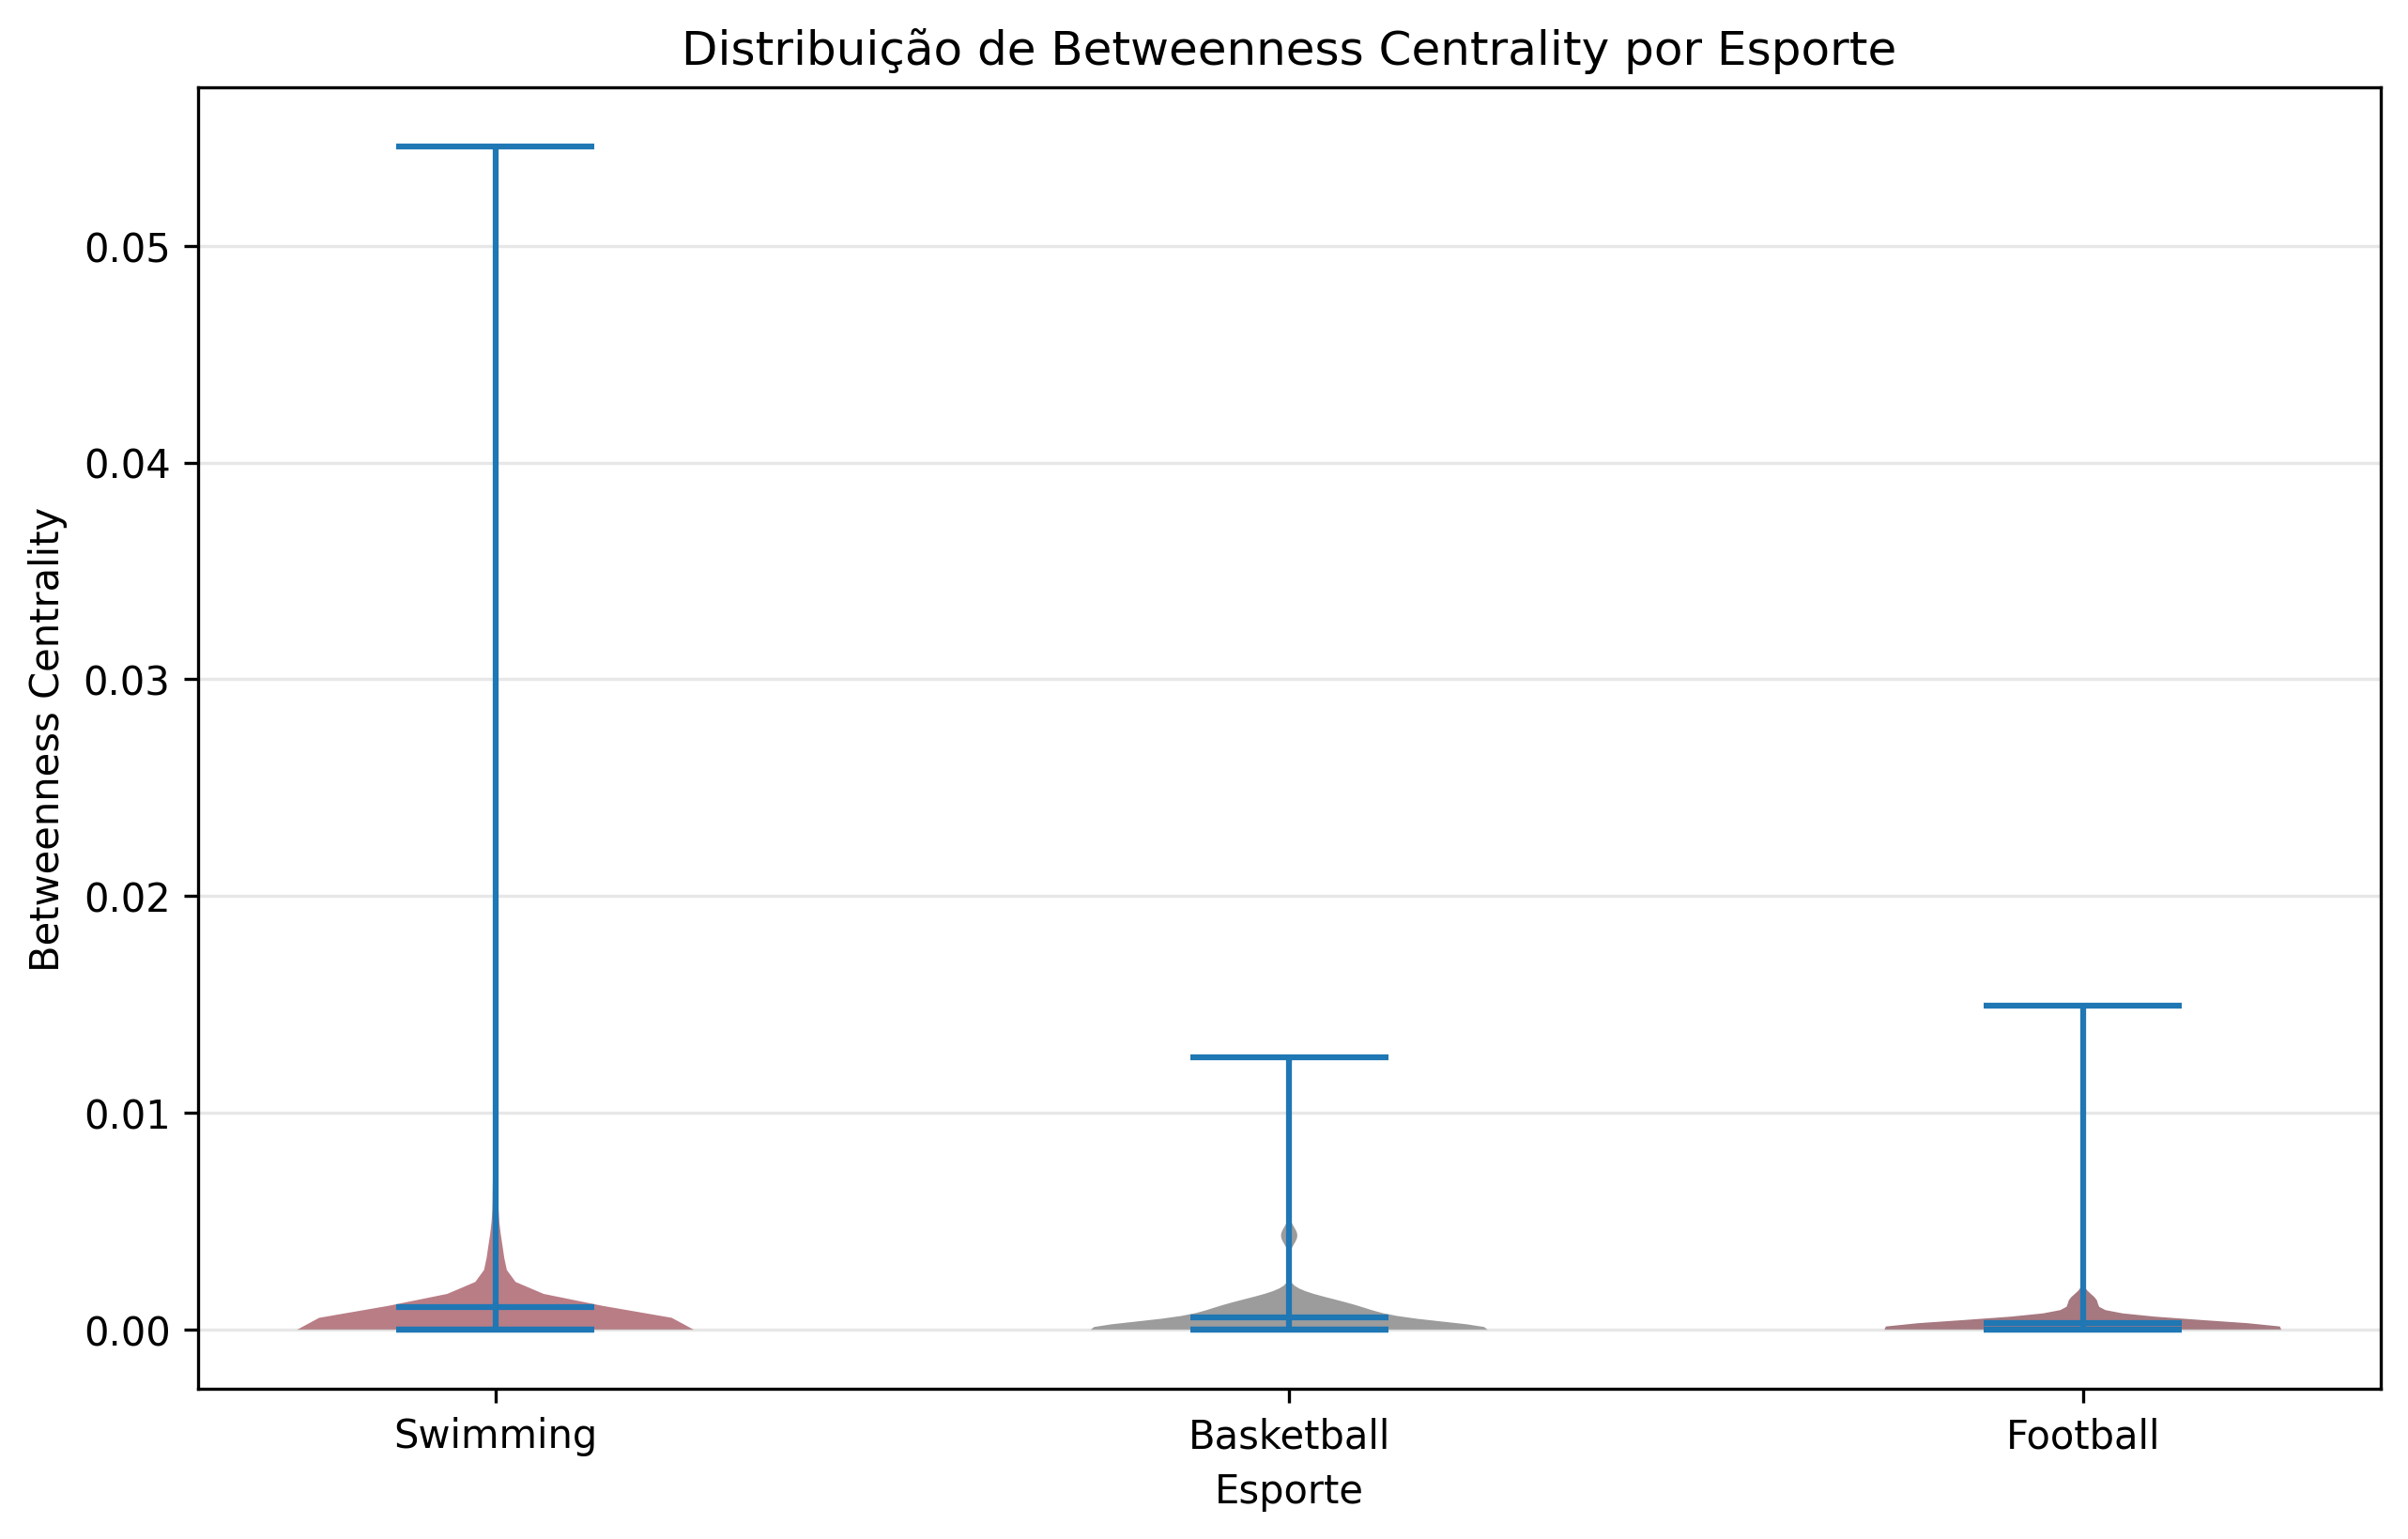
\includegraphics[width=\textwidth]{../monografia/figuras/fig_betweenness_violin.png}
        \end{column}
        \begin{column}{0.38\textwidth}
            \begin{block}{Definição}
                \footnotesize
                Atletas com alta betweenness conectam diferentes comunidades, atuando como \textbf{pontes estruturais}.
            \end{block}

            \vspace{0.2cm}
            \begin{block}{Distribuição}
                \footnotesize
                \begin{itemize}
                    \item \textbf{Swimming}: 10.2\% atletas-ponte
                    \item \textbf{Basketball}: 7.1\%
                    \item \textbf{Football}: 5.3\%
                \end{itemize}
            \end{block}

            \vspace{0.2cm}
            \begin{alertblock}{Interpretação}
                \footnotesize
                Natação apresenta maior proporção de atletas-ponte devido a estrutura modular com eventos individuais e revezamentos.
            \end{alertblock}
        \end{column}
    \end{columns}
\end{frame}
